\documentclass{beamer}
\usetheme[pageofpages=of,% String used between the current page and the
                         % total page count.
          bullet=circle,% Use circles instead of squares for bullets.
          titleline=true,% Show a line below the frame title.
          alternativetitlepage=true,% Use the fancy title page.
       %   titlepagelogo=logo-polito,% Logo for the first page.
       %   watermark=watermark-polito,% Watermark used in every page.
       %   watermarkheight=100px,% Height of the watermark.
       %   watermarkheightmult=4,% The watermark image is 4 times bigger
                                % than watermarkheight.
          ]{Torino}

\setbeamertemplate{footline}{
  \begin{beamercolorbox}[wd=\paperwidth,ht=1ex,dp=1ex]{footline}
    \vspace{5pt} \hspace{1em} \insertframenumber/\inserttotalframenumber
  \end{beamercolorbox}
}

\author{Brendon J. Brewer}
\title{STATS 331 -- Introduction to Bayesian Statistics}
\institute{The University of Auckland}
\date{}


\linespread{1.3}
\usepackage{minted}
\usepackage[utf8]{inputenc}
\usepackage{dsfont}
\newcommand{\given}{\,|\,}

\begin{document}

\frame{\titlepage}

\begin{frame}
\begin{center}
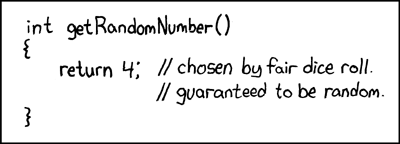
\includegraphics[width=0.6\textwidth]{images/random_number.png} \\

Credit: Randall Monroe, xkcd.com
\end{center}

\end{frame}

\begin{frame}
\begin{center}
\Large
Introduction to JAGS
\end{center}
\end{frame}


\begin{frame}
\frametitle{Introduction to JAGS}

\begin{itemize}
\item JAGS is a general purpose computer program for doing
MCMC sampling.\pause
\item It is useful for routine analyses (less useful for very large or
research problems).\pause
\item You tell it the prior, the sampling distribution, and the data and it will
do everything for you!\pause
\item It uses methods other than Metropolis (Gibbs sampling,
slice sampling, ...).
\end{itemize}

\end{frame}


\begin{frame}
\frametitle{Alternatives to JAGS}

There are some other programs similar to JAGS. I will mention them here,
so that you've heard of them, but we will not use them in this course.

\begin{itemize}
\item WinBUGS and OpenBUGS are both very similar to JAGS (the former is very
old and only works on Microsoft Windows).
Most of the time, code would not need to be modified to work in any of these.\pause
\item {\bf Stan} is a more modern and very popular package. It uses similar
ideas to JAGS, but its language is a bit different, and it uses a different,
more complex
MCMC sampler (based on {\bf Hamiltonian Monte Carlo}).
\end{itemize}

\end{frame}

\begin{frame}[fragile]
\frametitle{Installing JAGS}
You can install JAGS by first downloading it from this URL. Install it to
the default location on your system to avoid problems later.

\begin{center}
\url{https://mcmc-jags.sourceforge.io/}
\end{center}

\pause

After installing JAGS itself, you should install the \mintinline{r}{rjags}
package inside R:
\begin{minted}{r}
install.packages("rjags")
\end{minted}

\end{frame}


\begin{frame}[fragile]
\frametitle{The Bus Problem}
Recall the bus problem from the lecture notes. This was a binomial experiment
with $N=5$ trials, and the data was $x=2$ successes. The unknown parameter
is $\theta$, the success probability that applies on each trial.

\pause

We know how to solve this with a grid (Bayes Box), analytically (with a Beta
or Uniform prior for $\theta$), and with Metropolis.
How would we implement this in JAGS?

\end{frame}


\begin{frame}[fragile]
\frametitle{The Bus Problem in JAGS}

\begin{minted}{r}
model
{
    # The prior for the parameter
    theta ~ dunif(0, 1)

    # Sampling distribution (prior for the data!)
    x ~ dbin(theta, N)
}
\end{minted}

\end{frame}

\begin{frame}[fragile]
\frametitle{The Bus Problem in JAGS}
\begin{itemize}
\item We always write the assumptions inside the \mintinline{r}{model} block.\pause
\item We generally put the prior before the sampling distribution, but we don't
    actually have to!\pause
\item Quantities (either parameters or data) are defined into existence using
the tilde \mintinline{r}{~}.\pause
\item Note that $N$ is not defined anywhere --- this will be provided along
with the data value $x$.
\end{itemize}

\end{frame}

\begin{frame}[fragile]
\frametitle{Note About dbin() in JAGS}

\begin{itemize}
\item The distributions in JAGS are named similarly to the \mintinline{r}{d}
(density) functions in R, but not exactly the same --- here we see
\mintinline{r}{dbin()} whereas in R it's \mintinline{r}{dbinom()}.\pause
\item Also, people usually write Binomial$(N, p)$ or Binomial$(N, \theta)$,
but in JAGS the arguments are the other way around.\pause
\item There are some other quirks. E.g., for the normal distribution, the
second argument is {\em one over the variance}, i.e., we must write
\mintinline{r}{dnorm(mu, 1/sigma^2)}. 
We could write \mintinline{r}{dnorm(mu, 5)}
but the meaning of the second parameter is obscured.
\end{itemize}

\end{frame}



\begin{frame}[fragile]
\frametitle{Running JAGS from R}

\begin{itemize}
\item We will write R code that calls JAGS in the background using functions
from the \mintinline{r}{rjags} package.\pause
\item There is a script on Canvas called {\texttt use\_jags.R} which you can
use as a template.\pause
\item The JAGS model code is provided inside an R string.\pause
\item The data must be in an R list or data frame.\pause
\item After running the script, the results are put into a data frame called
\mintinline{r}{results}, whose (named) columns are the parameters.
\end{itemize}

\end{frame}



\end{document}

